 % reset section counter
%\setcounter{section}{0}
\metadata{8}{David Lin and Jinhui Wang}{Feb.~8th, 2021}

\sec{Covering number upper bounds Rademacher complexity}
In Chapter \ref{chap:gen-bounds}, we will prove Rademacher complexity bounds that hinge on elegant, ad-hoc algebraic manipulations that may not extend to more general settings. Here, we consider a more fundamental approach for proving empirical Rademacher complexity bounds based on coverings of the output space. The trade-off is generally more tedium.

The first important observation is that for purposes of computing the \textbf{empirical} Rademacher complexity on samples $z_1, ..., z_n$, 
\al{
    R_S(\cF) = \Exp_\sigma \sbr{\sup_{f \in \cF} \frac 1 n \sum_{i=1}^n \sigma_i f(z_i)},
}
we only care about the output of function $f \in \cF$, and not the function itself (i.e. it is sufficient for our purposes to know $f(z_1),\dots, f(z_n)$, but not know $f$). In other words, we can characterize $f \in \cF$ by $f(z_1),\dots, f(z_n)$. In the sequel, we will take advantage of this simplification from the (potentially large) space of all functions $\cF$ to the \textit{output space},
\begin{equation}
\cQ \triangleq \cbr{ \begin{pmatrix} f(z_1), \dots, f(z_n) \end{pmatrix}^\top: f\in \cF} \subseteq \R^n, \label{lec6:eqn:shattercoef}
\end{equation}
which may be drastically smaller than $\cF$. Correspondingly, the empirical Rademacher complexity can be rewritten as a maximization over the output space $\cQ$ instead of the function space $\cF$: 
\al{
    R_S(\cF) &= \Exp_\sigma \sbr{\sup_{v\in \cQ} \frac 1 n \inprod{\sigma, v}}.
}
In other words, the complexity of $\cF$ can be also interpreted as how much the vectors in $Q$ can be correlated with a random vector $\sigma.$ See Figure \ref{lec6:fig:rs-innerprod} for an illustration of this idea. One can also view $\Exp_\sigma \sbr{\sup_{v\in \cQ} \frac 1 n \inprod{\sigma, v}}$ as a complexity measure for the set $Q$. If we replace $\sigma$ by a Gaussian vector with spherical covariance, then the corresponding quantity (without the $\frac 1 n$ scaling), $\Exp_{g\sim N(0,I)} \sbr{\sup_{v\in \cQ} \inprod{g, v}}$, is often referred to as the Gaussian complexity of the set $Q$. (It turns out that Gaussian complexity and Rademacher complexity are closely related.)

Another corollary of this is that the empirical Rademacher complexity only depends on the functionality of $\cF$ but not on the exact parameterization of $\cF$ . For example, suppose we have two parameterizations $\cF = \left\{f(x)=\sum \theta_{i} x_{i} \mid \theta \in \mathbb{R}^{d}\right\}$ and $\cF' = \left\{f(x)=\sum \theta_{i}^{3} \cdot w_{i} x_{i} \mid \theta \in \R^{d}, w \in \mathbb{R}^{d}\right\}$. Since $Q_\cF$ and $Q_{\cF'}$ are the same, we see that $R_S(\cF) = R_S(\cF')$ since our earlier expression for $R_S(\cF)$ only depends on $\cF$ through $Q_\cF$. 

\begin{figure}[ht!]
	\begin{center}
		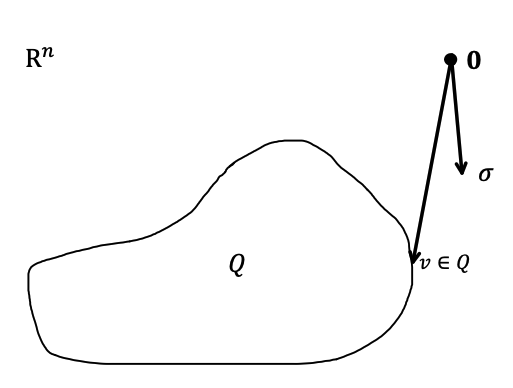
\includegraphics[width=.5\textwidth]{figures/remark2.png}
	\end{center}
	\caption{We can view empirical Rademacher complexity as the expectation of the maximum inner product between $\sigma$ and $v\in Q$.}
	\label{lec6:fig:rs-innerprod}
\end{figure}

\paragraph{Rademacher complexity of finite hypothesis classes.} In practice, we cannot directly evaluate the Rademacher complexity, so we instead bound its value using quantities that are computable. Given finite $|\cQ|$, we often rely on the following bound, which is also known as Masssart's finite lemma: 
\begin{proposition}
    Let $\cF$ be a collection of functions mapping $Z \mapsto \mathbb{R}$ and let $\cQ$ be defined as in \eqref{lec6:eqn:shattercoef}. Assume that $\frac{1}{\sqrt{n}} \norm{v}_2 \le M < \infty$ for all $v \in \cQ$. Then,
    \begin{align}
        R_S(\cF) \leq \sqrt{\frac{2 M^2 \log |\cQ|}{n}}
    \end{align}
    \label{lec6:prop:massartlemma}
\end{proposition}
We prove a (slightly) simplified version of this result in Problem 3(c) of Homework 2, so we omit the proof of Massart's lemma here. 

\begin{remark}
    Using Massart's lemma, we can bound the Rademacher complexity without referring to $\cQ$. Restating the assumption accordingly, we observe that if $\sqrt{\frac{1}{n}\sum_{i=1}^n f(z_i)^2} \le M$ for all $f \in \cF$, then $R_s(\cF) \le \sqrt{\frac{2M^2\log \abs{\cF}}{n}}$. Note that this corollary yields a looser bound than Massart's lemma since $|\cQ| \leq |\cF|$. 
\end{remark}
    
In practice, we rarely apply Massart's lemma directly since $|\cQ|$ is typically infinite. In the sequel, we discuss alternative approaches to bounding the Rademacher complexity that are appropriate for this setting.

\paragraph{Bounding Rademacher complexity using $\epsilon$-covers.}
When $|\cQ|$ is infinite, we can apply the same discretization trick that we used to prove the generalization bound for an infinite-hypothesis space. This time, instead of trying to cover the parameter space, we will cover the output space. To this end, we first recall a few definitions concerning $\epsilon$-covers.

\begin{definition}
$\cC$ is an \emph{$\epsilon$-cover} of $\cQ$ with respect to metric $\rho$ if for all $v' \in \cQ$, there exists $v \in \cC $ such that $\rho(v,v')\le \epsilon$.
\end{definition}

\begin{definition}
The \emph{covering number} is defined as the minimum size of an $\epsilon$-cover, or explicitly:
\begin{align}
    N(\epsilon, \cQ, \rho) \overset \triangle = (\text{min size of $\epsilon$-cover of $\cQ$ w.r.t.\ metric $\rho$}).
\end{align}
\end{definition}

\begin{figure}[h]
	\begin{center}
		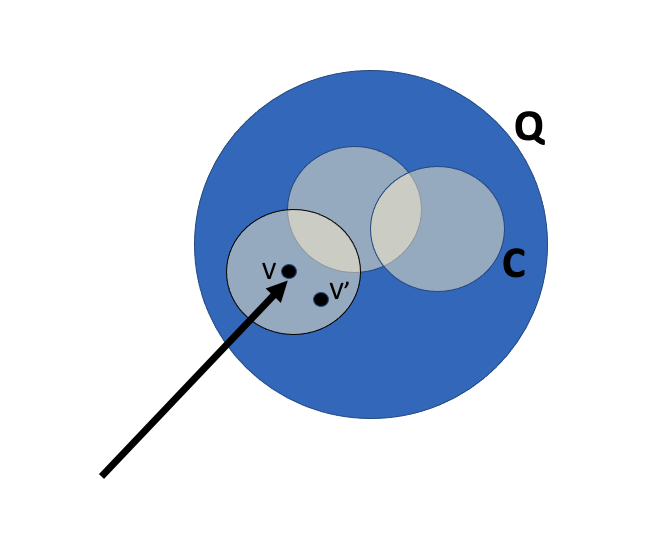
\includegraphics[width=.5\textwidth]{figures/onestep_bound.png}
	\end{center}
	\caption{We can visualize the $\epsilon$-cover $\cC$ by depicting a set of $\epsilon$-balls that cover the output space $\cQ$. The yellow circles denote the $\epsilon$-neighborhoods of the covering points $v \in \cC$.}
	\label{lec9:fig:eps-cover}
\end{figure}

In subsequent derivations, we will use the metric $\rho(v,v') = \frac 1 {\sqrt{n}} \norm{v-v'}_2$. 

\begin{remark}
We normalize the $\ell_2$ norm in $\rho$ by $\frac{1}{\sqrt{n}}$ to simplify comparisons to the functional analysis view of the Rademacher complexity. In the literature, the $\epsilon$-cover of $\cQ$ defined above is also referred to as an $\epsilon$-cover of the function class $\cF$ under the $L_2[P_n]$ metric.\footnote{$P_n$ denotes the empirical distribution, i.e. the uniform distribution over the observations $z_1,\dots,z_n$. More generally the $L_p[Q]$ metric is defined by $\Exp_Q \left [\left (f(z) - f'(z) \right )^p \right]^{1/p}$.} In particular, 
\begin{align}
L_2[P_n](f,f') = \sqrt{ \frac 1 n \sum_{i=1}^n (f(z_i) - f'(z_i))^2 }.
\end{align}
Recall we have established the following correspondences between the set of functions $\cF$ and the output space $\cQ$:
\begin{align}
    f \in \cF \iff \begin{pmatrix} f(z_1) \\ \vdots \\ f(z_n) \end{pmatrix} \in \cQ
\end{align}

We can write a trivial correspondence between both the output and function class points of view as follows:
\begin{align}
N(\epsilon, \cF, L_2(P_n)) = N\left (\epsilon, \cQ, \frac{1}{\sqrt{n}} || \cdot ||_2 \right )
\end{align}
The results below will be stated in the function-space notation, but in the proofs we will shift to the $\cQ$-formulation for the sake of clarity.
In general, we prefer to reason about covering numbers on $\cQ$ as it is more natural to analyze vector spaces compared to function spaces.
\label{lec8:rmk:l2pncover}
\end{remark}

Equipped with the definition of minimal $\epsilon$-covers, we can prove the following Rademacher complexity bound:

\begin{theorem}\label{lec8:thm:rc-covering-bd}
Let $\cF$ be a family of functions $Z \mapsto [-1,1]$. Then
\begin{equation}
R_S(\cF) \le \inf_{\epsilon > 0} \rbr{ \epsilon + \sqrt{ \frac {2\log N(\epsilon, \cF, L_2[P_n])} n } }. \label{lec8:eqn:rc-covering-bd}
\end{equation}
\end{theorem}

The $\epsilon$ term can be thought of as the discretization error, while the second term follows from Proposition~\ref{lec6:prop:massartlemma}.

\begin{proof}
Fix any $\epsilon > 0$. Let $\cC$ be the minimal $\epsilon$-cover $\cC$ of $\cQ$ with respect to the metric $\rho(v,v') = \frac 1 {\sqrt{n}} \norm{v-v'}_2$. 

For every point $v\in \cQ$, $v=v'+z$, where $v'\in \cC$ and $z$ is small (specifically, $\frac 1 {\sqrt{n}} \norm{z}_2 \le \epsilon$). This gives
\al{
    \frac 1 n \inprod{v, \sigma} &= \frac 1 n \inprod{v',\sigma} + \frac 1 n \inprod{z, \sigma}\\
    &\le \frac 1 n \inprod{v', \sigma} + \frac 1 n \norm{z}_2 \norm{\sigma}_2 
        &&\text{(Cauchy-Schwarz)} \label{lec8:eqn:cs-step}\\
    &\le \frac 1 n \inprod{v', \sigma} + \epsilon.
        &&\text{(since $\norm{z}_2\le \sqrt{n}\epsilon$ and $\norm{\sigma}_2 \le \sqrt{n}$)}
}
Taking the expectation of the supremum on both sides of this inequality gives
\al{
    R_S(\cF) &= \Exp_\sigma \sbr{\sup_{v\in \cQ} \frac 1 n \inprod{v,\sigma} }\\
    &\le \Exp_\sigma \sbr{\sup_{v'\in \cC} \rbr{\frac 1 n \inprod{v',\sigma} + \epsilon}}\\ 
    &\le \epsilon + \sqrt{ \frac {2\log \abs{\cC}} n } &\text{(Proposition~\ref{lec6:prop:massartlemma})} \\
    &= \epsilon + \sqrt{ \frac {2\log N(\epsilon, \cQ , \rho)} n } \\
    &= \epsilon + \sqrt{ \frac {2\log N(\epsilon, \cF , L_2[P_n])} n } &\text{(Remark~\ref{lec8:rmk:l2pncover})}
}
Since the argument above holds for any $\epsilon > 0$, we can take the infimum over all $\epsilon$ to arrive at Equation \eqref{lec8:eqn:rc-covering-bd}.

\end{proof}

\sec{Chaining and Dudley's theorem}

While Theorem \ref{lec8:thm:rc-covering-bd} is useful, the bound in Equation \eqref{lec8:eqn:cs-step} is rarely tight as $z$ might not be perfectly correlated with $\sigma$. It is possible to obtain a stronger theorem by constructing a chained $\epsilon$-covering scheme. Specifically, when we decompose $v=v'+z$, we can construct a finer-grained covering of the ball $B(v',\epsilon)$, and then we can decompose $z$ into smaller components and so on (see Figure \ref{lec9:fig:chaining_diag} for an illustration).

Using this method of chaining, we can obtain the following (stronger) result:

\begin{theorem}[Dudley's Theorem]
If $\cF$ is a function class from $Z$ to $\R$, then
\begin{equation}
    R_S(\mathcal{F})\leq 12\int_{0}^{\infty}\sqrt{\frac{\log N(\epsilon, \mathcal{F}, L_2[P_n])}{n}}d\epsilon. \label{lec9:eqn:dudley}
\end{equation}
\end{theorem}

Note that this theorem does not require the functions to be bounded.

\begin{remark}

It is not obvious how \eqref{lec9:eqn:dudley} improves upon the one-step discretization bound given by \eqref{lec8:eqn:rc-covering-bd}. At a high level, we can interpret this bound as removing the discretization error term by averaging over different scales of $\epsilon$.  But before we can explicitly prove this claim, we motivate our approach. In the proof of Theorem~\ref{lec8:thm:rc-covering-bd}, we approximated $v$ with $v' + z$ where $v'$ is the closest point to $v$ in the minimal $\epsilon$-cover of $\cQ$, and $z$ is the vector between $v'$ and $v$. In particular,
\begin{equation}
    \frac 1 n \inprod{v, \sigma} = \frac 1 n \inprod{v', \sigma} + \frac 1 n \inprod{z, \sigma} \label{lec9:eqn:disc_decomp}
\end{equation}
The difficult term to deal with is the last one, $\frac 1 n \inprod{z, \sigma}$. In the previous derivation, we naively upper bounded $\inprod{z, \sigma}$ using Cauchy-Schwarz,
\begin{equation}
    \frac 1 n \inprod{z,\sigma} \le \frac{\norm{z}_2\cdot \norm{\sigma}_2} n,
\end{equation}
but this bound is only tight if $z$ is perfectly correlated with $\sigma$. We claim that such perfect correlation is unlikely. Recall that the output space is defined by possible outputs of $f \in \cF$ given $n$ inputs. Unless our function class is extremely expressive, the set of radius $\epsilon$ around $v'$ contained in $\cQ$ will only be a small subset of the $\epsilon$-ball centered at $v'$; thus, $\sup_{z} \frac{1}{n} \inprod{z, \sigma} \ll \frac{\norm{z}_2 \cdot \norm{\sigma}_2}{n}$.

To more tightly bound $\Exp \l[ \sup \frac 1 n \inprod{z,\sigma}\r]$, we repeat the $\epsilon$-covering argument again with a smaller choice of $\epsilon$. Intuitively, this  procedure amounts to decomposing $\inprod{z, \sigma}$ from \eqref{lec9:eqn:disc_decomp} into another pair of terms corresponding to the new $\epsilon$-cover and the discretization error. ``Chaining'' then repeats this decomposition countably many times. Putting this argument in terms of Rademacher complexity, we can think of each chaining iteration as bounding $R_S(B_{v} \cap \cQ)$ where $B_{v}$ denotes the $\epsilon$-ball around $v \in \cC$ for the $\epsilon$-cover $\cC$ defined in the previous iteration. This procedure is illustrated visually by Figure~\ref{lec9:fig:chaining_diag}, and we formalize this argument in the sequel.
\end{remark}

\begin{figure}[ht!]
    \centering
    \begin{subfigure}[t]{0.45\textwidth}
        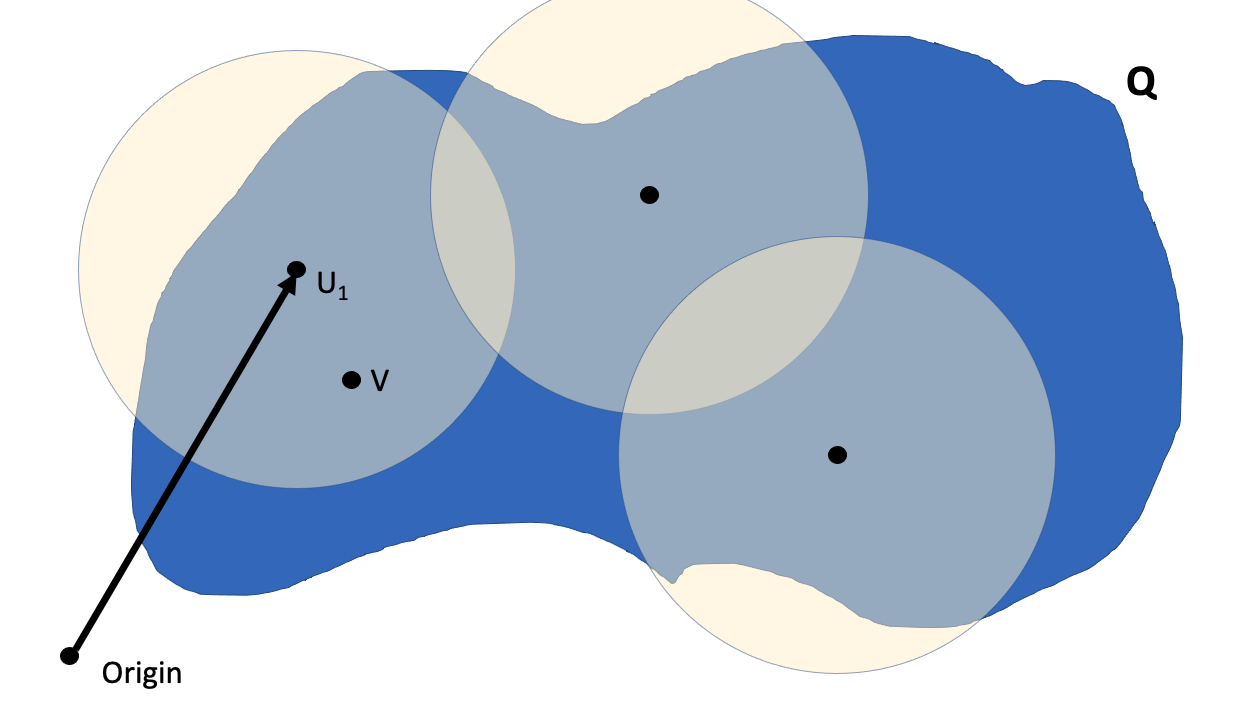
\includegraphics[width=\textwidth]{figures/chaining_1.png}
        \caption{}
        \label{lec9:fig:chaining_1}
    \end{subfigure}
    \hfill
    \begin{subfigure}[t]{0.45\textwidth}
        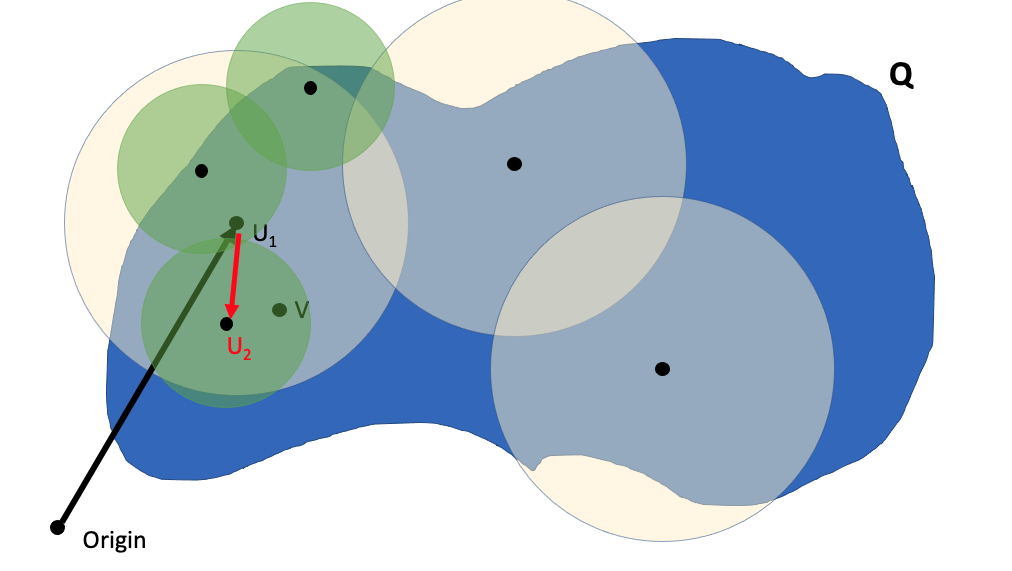
\includegraphics[width=\textwidth]{figures/chaining_2.png}
        \caption{}
        \label{lec9:fig:chaining_2}
    \end{subfigure}
    \hfill
    \begin{subfigure}[t]{0.45\textwidth}
        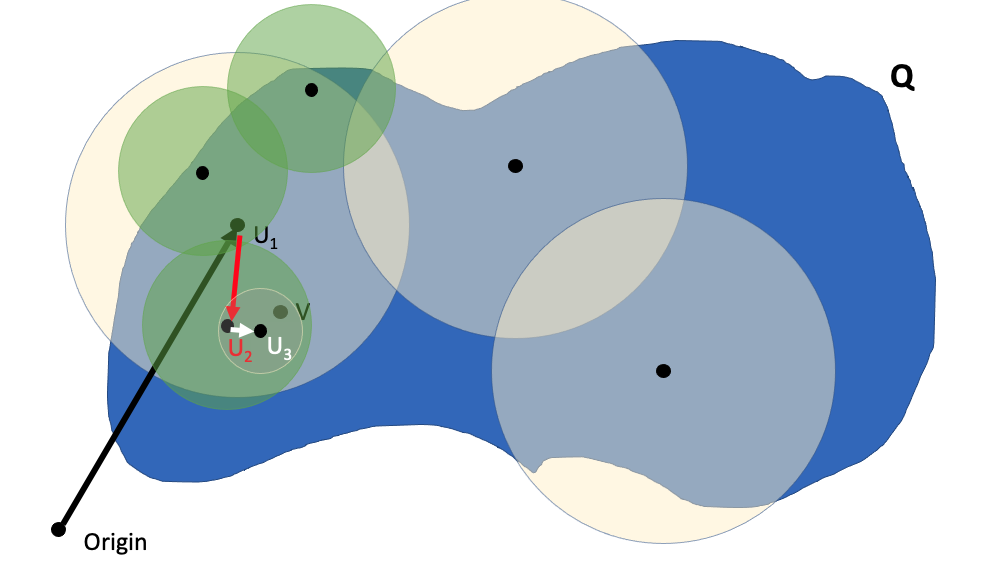
\includegraphics[width=\textwidth]{figures/chaining_3.png}
        \caption{}
        \label{lec9:fig:chaining_3}
    \end{subfigure}
    \caption{We depict how the chaining procedure approximates $v$ using a sequence of progressively finer discretizations. Figure~\ref{lec9:fig:chaining_1} illustrates how we first approximate $v$ using the nearest covering point $u_1$, while Figures~\ref{lec9:fig:chaining_2} and \ref{lec9:fig:chaining_3} describe how we refine this approximation using two finer covers, whose nearest points are denoted by $u_2$ and $u_3$, respectively.}
    \label{lec9:fig:chaining_diag}
\end{figure}

\begin{proof} 
    Let $\epsilon_0 = \sup_{f\in \cF} \max_i \abs{f(z_i)}$, so that for all $v \in \cQ$,
    \begin{equation}
        \epsilon_0 \ge \sqrt{\frac 1 n \sum_{i=1}^nf(z_i)^2}  = \sqrt{\frac 1 n \sum_{i=1}^n \norm{v}_2^2}.
    \end{equation}
    
    Define $\epsilon_j = 2^{-j}\epsilon_0$ and let $\cC_j$ be an $\epsilon_j$-cover of $\cQ$. Then, $\cC_0$ is the coarsest cover of $\cQ$, and as $j$ increases, we obtain progressively more fine-grained covers $\cC_j$. We use this sequence of covers to define a telescoping series that equals $v$; the terms in this series can then be analyzed using tools that we have developed in the prequel. 
    
    For $v \in \cQ$, let $\pi_i(v)$ denote the nearest neighbor of $v$ in $\cC_i$. Taking $\pi_0(v) = 0$, it follows from our definition of $\cC_i$ that
    \begin{align}
        v &= \pi_1(v) + \sum_{i = 2}^\infty (\pi_i(v) - \pi_{i - 1}(v)) \\
        &= \sum_{i = 1}^\infty (\pi_i(v) - \pi_{i - 1}(v)). \label{lec9:eqn:telescope_chain}
    \end{align}
    
    By definition, $\rho(v, \pi_i(v)) \le \epsilon_i$ and thus $\frac 1 {\sqrt n} \norm{v - \pi_i(v)}_2 \le \epsilon_i$. Substituting \eqref{lec9:eqn:telescope_chain} in the Rademacher complexity we aim to bound, we obtain
    \al{
        \Exp\l[\sup_{v \in \cQ} \frac 1 n \inprod{v, \sigma}\r]&= \Exp\l[\sup_{v \in \cQ} \frac 1 n \sum_{i=1}^\infty \inprod{\pi_i(v)-\pi_{i - 1}(v), \sigma}\r]\\
        &\le \Exp\l[\sum_{i=1}^\infty \sup_{u_i \in \cC_i, u_{i - 1} \in \cC_{i - 1}} \frac 1 n\inprod{u_i - u_{i - 1}, \sigma}\r]\\
        &= \sum_{i=1}^\infty \Exp\l[ \sup_{u_i \in \cC_i, u_{i - 1} \in \cC_{i - 1}} \frac 1 n\inprod{u_i - u_{i - 1}, \sigma}\r]. \label{lec9:eqn:chaining_expansion}
    }
    Observe that
    \begin{equation}
        \Exp\l[ \sup_{u_i \in \cC_i, u_{i - 1} \in \cC_{i - 1}} \frac 1 n\inprod{u_i-u_{i - 1}, \sigma}\r]
    \end{equation}
    is a Rademacher complexity defined over the \emph{finite} space $\cC_i \times \cC_{i - 1}$, so we can use Proposition~\ref{lec6:prop:massartlemma} (Massart's Lemma) to obtain a tractable upper bound. To do so, we must first compute an upper bound on $\frac{1}{\sqrt{n}} \norm{u_i - u_{i - 1}}_2$:
    \al{
        \frac 1 {\sqrt n} \norm{u_i - u_{i - 1}}_2 &= \frac 1 {\sqrt{n}} \norm{(u_i - v) - (u_{i - 1} - v)}_2\\
        &\le \frac 1 {\sqrt{n}} \l(\norm{u_i - v}_2 - \norm{u_{i - 1} - v}_2 \r)\\
        &\le \epsilon_i + \epsilon_{i - 1} \\
        &= 3 \epsilon_i & \text{($\epsilon_{i - 1} \defeq 2 \epsilon_i$)}
    }
    Now we apply Proposition~\ref{lec6:prop:massartlemma} with $M = 3 \epsilon_i$ and $\abs{\cQ} = \abs{\cC_i \times \cC_{i - 1}} \leq \abs{\cC_i} \cdot \abs{\cC_{i - 1}}$.
    \al{
        \Exp\l[\sup_{u_i \in \cC_i, u_{i - 1} \in \cC_{i - 1}} \frac 1 n \inprod{u_i - u_{i - 1}, \sigma} \r] & \le \sqrt{\frac{2(3 \epsilon_i)^2\log (\abs{\cC_i}\cdot \abs{\cC_{i-1}})}{n}}\\
        &= \frac{3 \epsilon_i}{\sqrt{n}}\sqrt{2(\log \abs{\cC_i} + \log \abs{\cC_{i-1}})}\\
        &\le \frac{6 \epsilon_i}{\sqrt{n}}\sqrt{\log \abs{\cC_i}} & (\abs{\cC_i} \ge \abs{\cC_{i - 1}}) \label{lec9:eqn:massartbound}
    }
    
    Applying \eqref{lec9:eqn:massartbound} to each term in \eqref{lec9:eqn:chaining_expansion} and substituting the covering number $N(\epsilon_i, \cF, L_2[P_n])$ for $|\cC_i|$, we obtain the following upper bound on the Rademacher complexity:
    \al{
        \Exp\l[\sup_{v \in \cQ} \frac 1 n \inprod{v, \sigma} \r] & \le \sum_{i = 1}^\infty \frac{6 \epsilon_i}{\sqrt{n}}\sqrt{\log N(\epsilon_i, \cF, L_2[P_n])}. \label{lec9:eqn:dudley_sumbound}
    }
    
    Recognizing that $\epsilon_i - \epsilon_{i + 1} = \frac{\epsilon_i}{2}$, we can rewrite \eqref{lec9:eqn:dudley_sumbound} as a right Riemann sum. In particular,
    \begin{align}
        \sum_{i = 1}^\infty \frac{6 \epsilon_i}{\sqrt{n}}\sqrt{\log N(\epsilon_i, \cF, L_2[P_n])} &= \frac{12}{\sqrt{n}} \sum_{i = 1}^\infty (\epsilon_i - \epsilon_{i + 1}) \sqrt{\log N(\epsilon_i, \cF, L_2[P_n])} \label{lec9:eqn:dudley_rriemann} \\
        &\le \frac{12}{\sqrt{n}} \int_{0}^{\epsilon_0} \sqrt{\log N(\epsilon, \cF, L_2[P_n])} d\epsilon, \label{lec9:eqn:dudley_almost}
    \end{align}
    where the last step follows by observing that $\log N(\epsilon, \cF, L_2[P_n])$ is decreasing in $\epsilon$. The monotonicity of $\log N(\epsilon, \cF, L_2[P_n])$ is also illustrated in Figure~\ref{lec9:fig:chaining_riemann}.

    \begin{figure}[h!]
        \begin{center}
            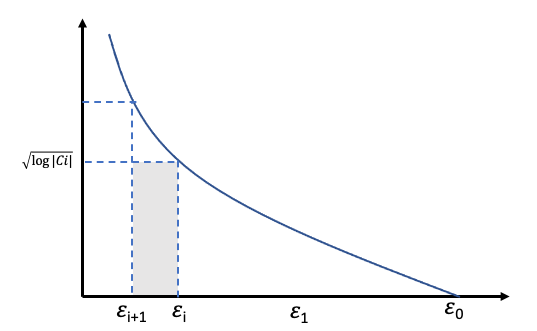
\includegraphics[width=.6\textwidth]{figures/chaining_riemann.png}
        \end{center}
        \caption{We observe that $\log N(\epsilon, \cF, L_2[P_n])$ is monotone decreasing in $\epsilon$. As a result, the right Riemann sum in \eqref{lec9:eqn:dudley_rriemann} will be upper bounded by the integral.}
        \label{lec9:fig:chaining_riemann}
    \end{figure}    

    To complete the proof, observe that $\log N(\epsilon, \cF, L_2[P_n]) = 0$ for all $\epsilon > \epsilon_0$. This allows us to extend the upper limit of the integral given by \eqref{lec9:eqn:dudley_almost} to $\infty$ and yields the desired result:
    \begin{align}
        \Exp\l[\sup_{v \in \cQ} \frac 1 n \inprod{v, \sigma} \r] & \le \frac{12}{\sqrt{n}} \int_{0}^\infty \sqrt{\log N(\epsilon, \cF, L_2[P_n])} d\epsilon.
    \end{align}
\end{proof}

\begin{remark}
If $\mathcal{F}$ consists of functions bounded in $[-1,1]$, then, we have that for all $\epsilon > 1, N(\epsilon, \mathcal{F}, L_2[P_n])=1$. To see this choose $\{f\equiv 0\}$, which is a complete cover for $\epsilon>1$. Hence, the limits of integration in \eqref{lec9:eqn:dudley} can be truncated to $[0,1]$:
    
    \begin{equation}
    R_S(\mathcal{F})\leq 12\int_{0}^{1}\sqrt{\frac{\log N(\epsilon, \mathcal{F}, L_2[P_n])}{n}}d\epsilon,
    \end{equation}
    
since $\log N(\epsilon, \mathcal{F}, L_2[P_n])=0$ for $\epsilon >1$.
\end{remark}

\subsec{Covering number regimes for which Dudley's theorem is finite}

Of course, the bound in \eqref{lec9:eqn:dudley} is only useful if the integral on the RHS is finite. Here are some setups where this is the case (we continue to assume that the functions in $\cF$ are bounded in $[-1, 1]$):

\begin{enumerate}
\item If $N(\epsilon, \mathcal{F}, L_2[P_n])\approx (1 / \epsilon)^R$ (ignoring multiplicative and additive constants), then we have $\log N(\epsilon, \mathcal{F}, L_2[P_n]) \approx  R\log (1/\epsilon)$. We can plug this into the RHS of \eqref{lec9:eqn:dudley} to get
        
\begin{equation}
\int_{0}^{1}\sqrt{\frac{\log N(\epsilon, \mathcal{F}, L_2[P_n])}{n}}d\epsilon = \int_{0}^1\sqrt{\frac{R\log(1/\epsilon)}{n}}d\epsilon \approx \sqrt{\frac{R}{n}}.
\end{equation}
            
\item If the covering number has the form $N(\epsilon, \mathcal{F}, L_2[P_n])\approx a^{R/\epsilon}$ for some $a$, then we have $\log N(\epsilon, \mathcal{F}, L_2[P_n]) \approx \frac{R}{\epsilon}\log a$. The bound in \eqref{lec9:eqn:dudley} becomes
        
\begin{align}
\int_0^1\!\!\sqrt{\frac{\log N(\epsilon, \mathcal{F}, L_2[P_n])}{n}}d\epsilon &\approx \int_0^1\!\!\sqrt{\frac{R}{n\epsilon}\log a}\, d\epsilon \\
&= \sqrt{\frac{R}{n}\log a} \int_0^1\!\!\sqrt{\frac{1}{\epsilon}}d\epsilon \\
&= \tilO \l(\sqrt{\frac{R}{n}}\r).
\end{align}
        
\item If the covering number has the form $N(\epsilon, \mathcal{F}, L_2[P_n])\approx a^{R/\epsilon^2}$, then $\log N(\epsilon, \mathcal{F}, L_2[P_n])\approx \frac{R}{\epsilon^2}\log a$. In this case we have:
        
\begin{equation}\int_0^1\sqrt{\frac{\log N(\epsilon, \mathcal{F}, L_2[P_n])}{n}}d\epsilon \approx \sqrt{\frac{R}{n}\log a} \underbrace{\int_0^1\frac{1}{\epsilon}d\epsilon}_{=\infty}=\infty,
\end{equation}

i.e. the bound in \eqref{lec9:eqn:dudley} is vacuous. This is because of the behavior of $\epsilon \mapsto 1/\epsilon^2$ near 0: the function goes to infinity too quickly for us to upper bound its integral. Fortunately, there is an ``improved'' version of Dudley's theorem that is applicable here:
        
\begin{theorem}[Localized Dudley's Theorem]\label{lec9:thm:better-dudley}
If $\cF$ is a function class from $Z$ to $\R$, then for any fixed cutoff $\alpha \geq 0$ we have the bound
\begin{equation}\label{lec9:eqn:better-dudley}
R_S(\mathcal{F})\leq 4\alpha + 12\int_{\alpha}^{\infty}\sqrt{\frac{\log N(\epsilon, \mathcal{F}, L_2[P_n])}{n}}d\epsilon.      
\end{equation}
\end{theorem}
The proof of this theorem is similar to the proof of the original Dudley's theorem, except that the iterative covering procedure is stopped at the threshold $\epsilon = \alpha$ at the cost of the extra $4\alpha$ term above.
        
Theorem \ref{lec9:thm:better-dudley} allows us to avoid the problematic region around $\epsilon=0$ in the integral in \eqref{lec9:eqn:dudley}. If we let $\alpha = 1/\mathsf{poly}(n)$, where $\mathsf{poly}(n)$ denotes some polynomial function of $n$, the bound in \eqref{lec9:eqn:better-dudley} becomes
\begin{align}
R_S(\mathcal{F}) &\leq \frac{1}{\mathsf{poly}(n)} + \frac{\sqrt{R\log a}}{\sqrt{n}}\int_{\alpha}^1\frac{1}{\epsilon}d\epsilon \\
&= \frac{1}{\mathsf{poly}(n)}  + \frac{\sqrt{R\log a}}{\sqrt{n}} \log(1/\alpha) \\
&= \tilO \l(\sqrt{\frac{R}{n}}\r).
\end{align}
\end{enumerate}

In summary, we have that $R_S(\mathcal{F}) \leq \tilO\l(\sqrt{\frac{R}{n}}\r)$ for these three dependencies on $\epsilon$: when $\log N(\epsilon, \mathcal{F}, L_2[P_n]) \approx R\log (1/\epsilon),\ \frac{R}{\epsilon} \log a,\text{ or } \frac{R}{\epsilon^2} \log a$ for some $a$. Note that if the dependence on $\epsilon$ is $1/\epsilon^c$ for $c > 2$, then even the improved Dudley's theorem does not help us. This is because the $\log(1/\alpha)$ term above becomes $\alpha^{1-c/2}$, and when $\alpha = 1/\mathsf{poly}(n)$, this term leads to a bad dependence on $n$.

\subsec{Regimes where we can get covering number bounds}
The previous remarks discuss how strong our bounds on covering number need to be in order to get a useful result. Here we describe some situations in which we know how to obtain these covering number bounds, though we omit the proofs here.

First, consider the following covering number bound for linear models:

\begin{theorem}[\cite{zhang2002}]
Suppose $x^{(1)}, \cdots, x^{(n)} \in \mathbb{R}^d$ are $n$ data points, and $p, q$ satisfies $p^{-1} + q^{-1} = 1$ and $2 \le p \le \infty$. Assume that $||x^{(i)}||_p \le C$ for all $i$. Let:
\begin{align}
    F_q = \{x \to w^T x : ||w||_q \le B\}
\end{align}
and let $\rho = L_2[P_n]$. Then, $\log N(\epsilon, F_q, \rho) \le \l [\frac{B^2c^2}{\epsilon^2}\r ] \log_2 (2d + 1)$. When $p = 2, q = 2$, we further obtain that:
\begin{align}
    \log N(\epsilon, F_2, \rho) \le \l [\frac{B^2c^2}{\epsilon^2} \r ] \log_2 (2 \min (n, d ) + 1)
\end{align}
\end{theorem}
\begin{remark}
Using the covering number bound derived above, it is also possible to show that the Rademacher complexity of this class of linear models is bounded by
\begin{align}
    R_s(F_q) &\le \tilO{\left( \frac{BC}{\sqrt{n}} \right)}
\end{align} 
\end{remark}
For multivariate linear functions, let $\norm{M^T}_{2,1}$ denote the sum of the $\ell_2$ norms of the $n$ rows of $M$ where $M = (M_1, \cdots, M_n) \in \mathbb{R}^{m \times n}$. 
\begin{theorem}
Let $\cF = \{x \to Wx : W \in \mathbb{R}^{m \times d}, ||W^T||_{2, 1} \le B\}$ and let $C = \sqrt{\frac{1}{n} \sum_{i = 1}^n ||x^{(i)}||_2^2}$. Then, 
\begin{equation}
\log N(\epsilon, F, L_2(P_n)) \le \l [\frac{c^2B^2}{\epsilon^2} \r ] \log (2dm).
\end{equation}
\end{theorem}

Covering numbers also interact nicely with composition by Lipschitz functions. The following result is the analog of Talagrand's lemma for covering numbers.
\begin{lemma} Suppose $\phi$ is $\kappa$-Lipschitz, and $\rho = L_2[P_n]$. Then,
    \begin{align}
        \log N(\epsilon, \phi \circ \cF, \rho) \le \log N(\epsilon / \kappa, \cF, \rho) \label{lec9:eqn:covering-num-lipschitz}
    \end{align}
\end{lemma}
\begin{proof}
Let $\cC$ denote an $\epsilon/\kappa$-cover for $\cF$. Then $\phi \circ \cC$ is an $\epsilon$-cover of $\phi \circ \cF$.
\begin{align}
\rho(\phi \circ f', \phi \circ f) &= \sqrt{\frac{1}{n} \sum (\phi(f'(z_i)) - \phi(f(z_i)))^2} \\ 
&\le \sqrt{\frac{1}{n} \cdot \kappa^2 \sum(f'(z_i) - f(z_i))^2}\\
&\le \kappa \cdot \frac{\epsilon}{\kappa} = \epsilon
\end{align}
\end{proof}

Using these results, we can obtain a bound on the Rademacher complexity of a dense neural network. Consider a deep network
\begin{equation}
f(x) = W_r\sigma(W_{r-1}\sigma(\cdots \sigma(W_1x)\ldots),
\end{equation}

where $W_i$ are layer-wise weights and $\sigma$ is an activation function which is 1-Lipschitz. For this setup we have the following Rademacher complexity bound:
\begin{equation}
R_S (\cF) \leq \underbrace{\l(\prod_{i=1}^r\|W_i\|_{\textup{op}} \r)}_{\text{relatively large}} \cdot \underbrace{\l( \sum_{i=1}^r\frac{\|W_i^\top\|^{2/3}_{2,1}}{\|W_i\|_{\textup{op}}^{2/3}}\r)^{3/2}}_{\text{relatively small}}.
\end{equation}
        
Here $\|W\|_{\textup{op}}$ is the operator norm (or spectral norm) of $W$, and $\|W_i^\top\|_{2,1}$ denotes the sum of the $l_2$ norms of the rows of $W_i$. The second term is relatively small as it is a sum of matrix norms, and so the bound is dominated by the first term, which is a product of matrix norms. This first term comes from composition of Lipschitz functions as in \eqref{lec9:eqn:covering-num-lipschitz} above, since the Lipschitz constant of a linear operator is its spectral norm. The full details are presented in \cite{bartlett2017}.


\sec{VC dimension and its limitations}
We will focus on classification and will be working within the framework of supervised learning stated in Chapter \ref{chap:supervised}. The labels belong to the output space $\mathcal{Y} = \{-1, 1\}$, each classifier is a function $h:\mathcal{X}\to\R$ for all $h \in \cH$, and the prediction is the sign of the output, i.e. $\hat{y} = \sgn(h(x))$. We will look at zero-one loss, i.e. $\err((x,y), h) = \mathbbm{1}(\sgn(h(x))\neq y)$. Note that we can re-express the loss function as
\begin{equation}
\err((x,y), h) = \frac{1-\sgn(h(x))y}{2}.
\end{equation}

The first approach is to reason directly about the Rademacher complexity of $\err$ loss, i.e. considering the family of functions $\cF = \left\{ z = (x, y) \mapsto \err((x, y), h) : h \in \cH \right\}$. Define $Q$ to be the set of all possible outputs on our dataset: $Q=\left\{\left(\sgn\left(h\left(x^{(1)}\right)\right), \dots, \sgn \left(h\left(x^{(n)}\right)\right)\right)\mid  h \in \cH \right\}$. Then, using our earlier remark about viewing the empirical Rademacher complexity as an inner product between $v\in Q$ and $\sigma$, we have
\begin{align}
R_S(\cF) &= \Exp_{\sigma_1,\dots, \sigma_n} \l[ \sup_{f\in \cF} \frac{1}{n} \sum^n_{i=1} \sigma_i \frac{1-\sgn(h(x^{(i)}))y_i}{2} \r] \\
&= \Exp_{\sigma_1,\dots, \sigma_n} \l[ \sup_{f\in \cF} \frac{1}{n} \sum^n_{i=1} \sigma_i \frac{\sgn(h(x^{(i)}))}{2} \r] \\
&= \frac{1}{2}\Exp_{\sigma_1,\dots, \sigma_n} \l[ \sup_{v\in Q} \frac{1}{n} \langle \sigma, v\rangle \r].
\end{align}

Notice that the supremum is now over $Q$ instead of $\cF$. If $n$ is sufficiently large, then it is typically the case that $|Q|>|\cF|$. To see why this is the case, note that each function $f$ corresponds to a single element in $Q$. However, as $n$ increases, $|Q|$ increases as well. For any particular $v\in Q$, notice that $\langle v, \sigma\rangle$ is a sum of bounded random variables, so we can use Hoeffding's inequality to obtain
\begin{equation}
\Pr\left[\frac{1}{n}\langle\sigma, v\rangle\geq t\right] \leq \exp (-n t^2 / 2).
\end{equation}
Taking the union bound over $v\in Q$, we see that 
\begin{equation}
\Pr\left[\exists v\in Q \text{ such that } \frac{1}{n}\langle\sigma, v\rangle \geq t\right] \leq |Q| \exp (-nt^2 / 2).
\end{equation}
Thus, with probability at least $1-\delta$, it is true that $\sup _{v \in Q} \frac{1}{n}\langle v, \sigma \rangle \leq \sqrt{\frac{2(\log|Q| + \log (2/\delta))}{n}}$. Similarly, we can show that $\Exp \left[ \sup _{v \in Q} \frac{1}{n}\langle v, \sigma \rangle \right] \leq O\l(\sqrt{\frac{\log|Q| + \log (2/\delta)}{n}}\r)$ holds.

The key point to notice here is that the upper bound on $R_S(\cF)$ depends on $\log |Q|$. \textit{VC dimension} is one way that we deal with bounding the size of $Q$ We will not delve into the details of this approach (for those interested, see Section 3.11 of \cite{percynotes}). VC dimension, however, has a number of limitations. For one, we will always end up with a bound that depends somehow on the dimension. For linear models, we obtain a bound $\log |Q| \lesssim d \log n$, corresponding to a bound on Rademacher complexity that looks like
\begin{equation}
R_S(\cF) \leq \tilO \left( \sqrt{\frac{d}{n}} \right),
\end{equation}
so we still have a $\sqrt{d}$ term. This will not be a good bound for high-dimensional models. For general models, we will arrive a bound of the form 
\begin{equation}
R_S(\cF) \leq \tilO \left( \sqrt{\frac{\text{\# of parameters}}{n}} \right).
\end{equation}
This upper bound only depends on the number of parameters in our model, and does not take into the account the scale and norm of the parameters. Additionally, this doesn't work with kernel methods since the explicit parameterization is possibly infinite-dimensional, and therefore this upper bound becomes useless.

These limitations motivation the use of margin theory, which does take into account the norm of parameters and provides a theoretical basis for regularization techniques such as $L_1$ and $L_2$ regularization.